\documentclass{article}

\usepackage{graphicx}
\usepackage{tikz}
\usepackage{tikzsymbols}
\usetikzlibrary{calc,patterns,shapes.geometric}
\pagestyle{empty}
\usepackage[margin=0pt]{geometry}
\geometry{papersize={14in,12in}}

\def\centerarc[#1](#2)(#3:#4:#5){\draw[#1] ($(#2)+({#5*cos(#3)},{#5*sin(#3)})$) arc (#3:#4:#5);}

\begin{document}
	\begin{figure}
		\centering
		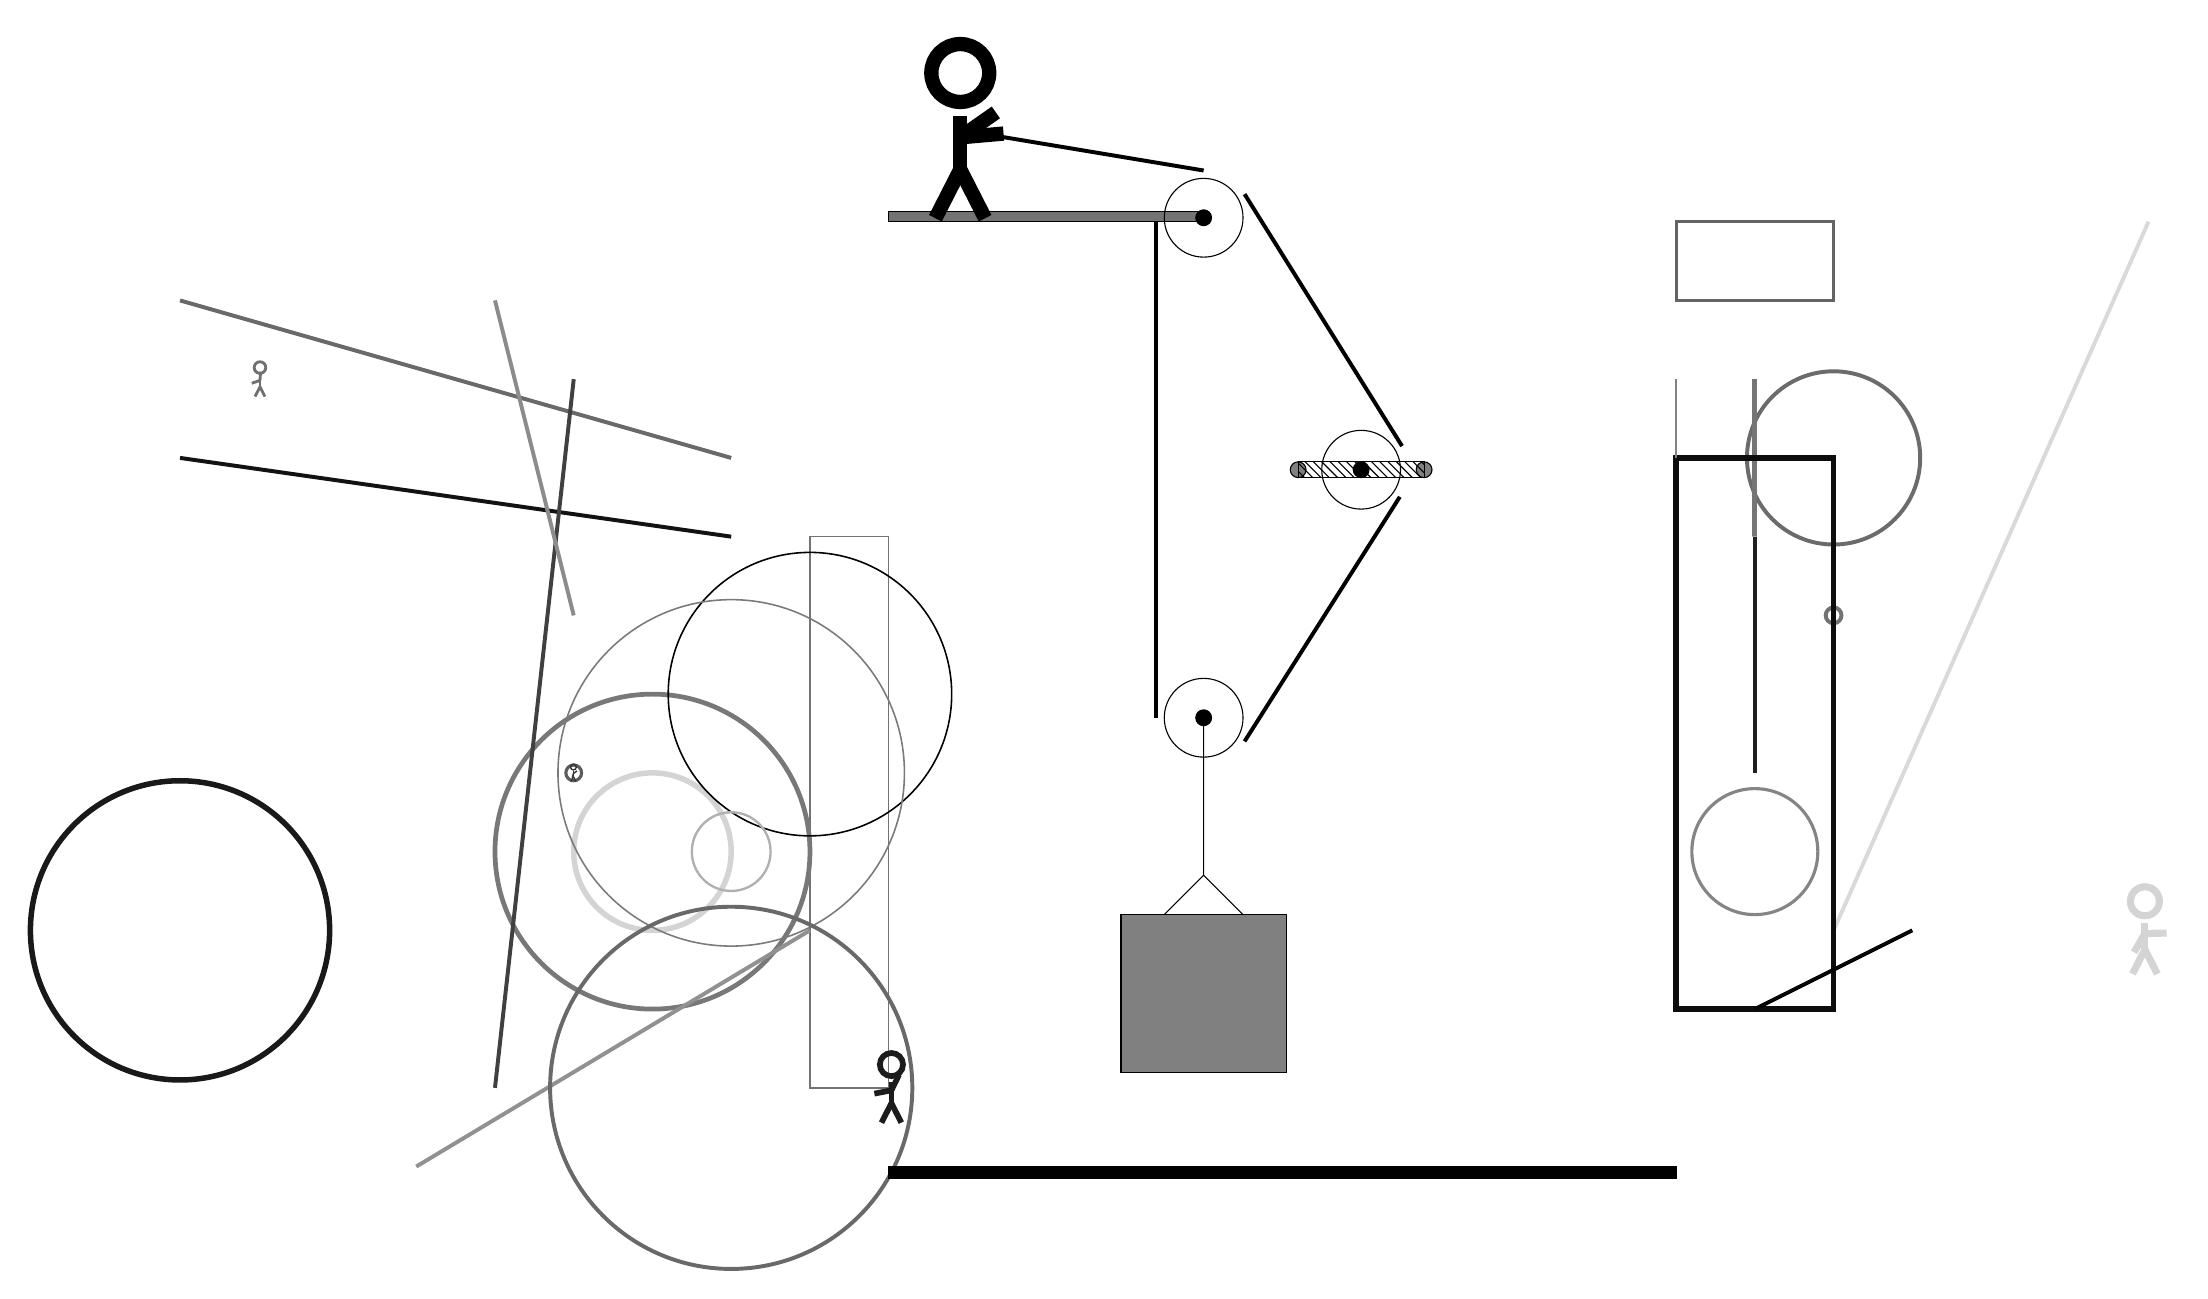
\begin{tikzpicture}
			%%%%% START %%%%%
			
			\draw[fill=black!55] (-2, 9) rectangle (2, 9.125);
			
			\draw (2, 2.7) circle (0.5);
			\draw[fill=black] (2, 2.7) circle (0.1);
			
			\draw (2, 9.05) circle (0.5);
			\draw[fill=black] (2, 9.05) circle (0.1);
			
			\draw[fill=white](4, 5.85) circle (0.5);
			\draw[fill=black] (4, 5.85) circle (0.1);
			\draw[fill=black!50] (3.2, 5.85) circle (0.1);
			\draw[fill=black!50] (4.8, 5.85) circle (0.1);
			\draw[pattern=north west lines, pattern color=black] (3.2, 5.95) rectangle (4.8, 5.75);
			
			\draw (2, 2.7) -- (2, 0.7) -- (1.5, 0.2) -- (2.5, 0.2) -- (2, 0.7);
			\draw[fill=black!50] (0.95, 0.2) rectangle (3.05, -1.8);
			
			\draw[line width=0.7mm, color=black!27] (9, -2) rectangle (9, -2);
			
			\node[line width=0.2mm, color=black!17] at (14, 0) {\Strichmaxerl[5][60][1]};
			\draw[line width=0.2mm, color=black!55] (-2, -2) rectangle (-3, 5);
			\draw [line width=0.4mm, color=black!64](-6, 2) circle (0.1);
			\draw [line width=0.6mm, color=black!53](-5, 1) circle (2.0);
			
			\draw[line width=0.5mm, color=black!15](10, 0) -- (14, 9);
			\draw[line width=0.5mm, color=black!93](-4, 5) -- (-11, 6);
			\draw[line width=0.5mm, color=black!59](-4, 6) -- (-11, 8);
			\draw[line width=0.5mm, color=black!43](-3, 0) -- (-8, -3);
			
			\draw[line width=0.5mm, color=black!75](-7, -2) -- (-6, 7);
			
			\draw [line width=0.5mm, color=black!55](10, 4) circle (0.1);
			
			\draw [line width=0.5mm, color=black!58](10, 6) circle (1.1);
			\draw [line width=0.7mm, color=black!17](-5, 1) circle (1.0);
			\draw[line width=0.5mm, color=black!88](9, 5) -- (9, 2);
			\draw[line width=0.6mm, color=black!54] (9, 5) rectangle (9, 7);
			\draw [line width=0.2mm, color=black!100](-3, 3) circle (1.8);
			
			\draw[line width=0.7mm, color=black!95] (8, 6) rectangle (10, -1);
			\draw[line width=0.5mm, color=black!45](-7, 8) -- (-6, 4);
			\node[line width=0.5mm, color=black!79] at (-6, 2) {\Strichmaxerl[1][75][36]};
			\draw[line width=0.5mm, color=black!98](9, -1) -- (11, 0);
			\draw [line width=0.2mm, color=black!52](-4, 2) circle (2.2);
			
			\draw [line width=0.7mm, color=black!90](-11, 0) circle (1.9);
			\draw[line width=0.4mm, color=black!61] (8, 8) rectangle (10, 9);
			\node[line width=0.3mm, color=black!89] at (-2, -2) {\Strichmaxerl[4][11][64]};
			\draw[line width=0.2mm, color=black!49] (8, 6) rectangle (8, 7);
			\draw [line width=0.5mm, color=black!59](-4, -2) circle (2.3);
			
			\node[line width=0.5mm, color=black!56] at (-10, 7) {\Strichmaxerl[2][19][86]};
			\draw [line width=0.4mm, color=black!48](9, 1) circle (0.8);
			
			\draw [line width=0.3mm, color=black!31](-4, 1) circle (0.5);
			
			\draw[line width=0.5mm] (1.4, 9) -- (1.4, 2.7);
			\centerarc[line width=0.5mm](2, 2.7)(180:330:0.6);
			\draw[line width=0.5mm](2.5196, 2.4) -- (4.4915, 5.5058);
			\centerarc[line width=0.5mm](4, 5.85)(390:325:0.6);
			\draw[line width=0.5mm](4.5196, 6.15) -- (2.5196, 9.35);
			\centerarc[line width=0.5mm](2, 9.05)(30:90:0.6);
			\draw[line width=0.5mm](2, 9.65) -- (-1, 10.15);
			
			\node at (-1, 10.15) {\Strichmaxerl[10][-175][35]};
			
			\draw[fill=black] (-2, -3) rectangle (8, -3.15);
			
			%%%%% END %%%%%
		\end{tikzpicture}
	\end{figure}	
\end{document}